\documentclass{article}
% For math environments
\usepackage{amsmath, amsfonts}
% For links
\usepackage[colorlinks=true,
    linkcolor = blue,
    urlcolor  = blue,
    citecolor = blue,
    anchorcolor = blue]{hyperref}
% Put space between paragraphs
\usepackage{parskip}
% For figures
\usepackage{tikz}
% Set the margins to not be ridiculous
\usepackage[margin=0.75in]{geometry}
% For multiple columns
\usepackage{multicol}
% For controlling enum/itemize spacing and indentation
\usepackage{enumitem}
% More math symbols
\usepackage{amssymb}
% To change enumerate labels

% For tikz plots
\usepackage{pgfplots}
% This isn't needed but avoids a compiler warning
\pgfplotsset{compat=1.16}

% Allow multi-line equations to be broken across pages
\allowdisplaybreaks

% Use @ as a letter
\makeatletter

% Scale down all tikz coordinates while maintaining font size
\tikzset{every picture/.style={scale=0.45, every picture/.style={}}}


% Macros
% Monospace code
\def\code#1{\texttt{#1}}

% Greek letters
\def\a{\alpha}
\def\b{\beta}
\def\g{\gamma}
\def\d{\delta}
\def\D{\Delta}

% Commands that make life easier
\newcommand\gath[1]{\begin{gather} #1 \end{gather}}
\newcommand\ali[1]{\begin{align} #1 \end{align}}
\newcommand\parens[1]{\left( #1 \right)}
\newcommand\squares[1]{\left[ #1 \right]}
\newcommand\braces[1]{\left\{ #1 \right\}}
\newcommand\angles[1]{\left\langle #1 \right\rangle}
\newcommand\deriv[2]{\frac{d #1}{d #2}}
\newcommand\abs[1]{\left| #1 \right|}
\newcommand\floor[1]{\left\lfloor #1 \right\rfloor}
\DeclareMathOperator{\lcm}{lcm}
\def\non{\nonumber \\}

% Multiline equation space
\def\mlesp{\hspace{1.2cm}}

% For grid diagrams
\newcommand\gridbox[3]{\draw (#1,#2) rectangle (#1+1,#2+1) node[pos=.5] {#3};}
\newcommand\gridboxh[3]{\draw[fill=red!20] (#1,#2) rectangle (#1+1,#2+1) node[pos=.5] {#3};}
\newcommand\gridboxb[3]{\draw[fill=black] (#1,#2) rectangle (#1+1,#2+1) node[pos=.5] {#3};}
\newcommand\gridsym[3]{\node at (#1+0.5,#2+0.5) {$#3$};}
\newcommand\gridblank[2]{\filldraw[draw=gray, color=gray] (#1,#2) rectangle (#1+1,#2+1);}
\newcommand\gridcirc[2]{\draw (#1 + 0.5,#2 + 0.5) circle (0.25);}
\newcommand\cwlab[3]{
  \def\dd{0.15}
  \draw (#1 + \dd - 0.03, #2 + 1 - \dd) node {\scriptsize #3};
}

\def\bbw{3.5}
\def\bbh{2}
\newcommand\bigbox[3]{\draw (#1*\bbw,#2*\bbh) rectangle (#1*\bbw+\bbw,#2*\bbh+\bbh) node[pos=.5] {#3};}
\newcommand\bbtextr[3]{\node[right] at (#1*\bbw,#2*\bbh+0.5*\bbh) {#3};}
\newcommand\bbtextb[3]{\node[align=center] at (#1*\bbw+0.5*\bbw,#2*\bbh+0.5*\bbh) {#3};}

% Box puzzle stock answer
\newcommand\boxans[1]{
  Logic was used to deduce the solution:

  #1

  This was verified using Python as well as shown to be unique with a brute force approach.
}

% Multiple numbers
\newcommand\mn[1]{$#1$'s}

% Commands for problems
\newcommand\problem[4]{
  \section*{#1}

  Question: #3
  
  Answer: #2
  
  Explanation: #4
}
\newcommand\aproblem[4]{\problem{Dec #1}{#2}{#3}{#4}}
\newcommand\cproblem[4]{\problem{Problem #1}{#2}{#3}{#4}}

\def\advent@xxiv@i{
  Eve writes down five different positive integers.
  The sum of her integers is $16$. What is the product of her integers?
}

\def\advent@xxiv@ii{
  $14$ is the smallest even number that cannot be obtained by rolling two $6$-sided dice and finding the product of the numbers rolled.

  What is the smallest even number that cannot be obtained by rolling one hundred $100$-sided dice and finding the product of the numbers rolled?
}

\def\advent@xxiv@iii{
  There are $5$ ways to write $5$ as the sum of positive odd numbers:
  \begin{itemize}
    \item $1 + 1 + 1 + 1 + 1$
    \item $1 + 1 + 3$
    \item $3 + 1 + 1$
    \item $1 + 3 + 1$
    \item $5$
  \end{itemize}

  How many ways are there to write $14$ as the sum of positive odd numbers?
}

\def\advent@xxiv@iv{
  The geometric mean of a set of $n$ numbers is computed by mulitplying all the numbers together, then taking the $n$th root.
  The factors of $9$ are $1$, $3$, and $9$.
  The geometric mean of these factors is
  \gath{
    \sqrt[3]{1 \times 3 \times 9} = \sqrt[3]{27} = 3
  }
  What is the smallest number where the geometric mean of its factors is $13$?
}

\def\advent@xxiv@v{
  The sum of $11$ consecutive integers is $2024$.
  What is the smallest of the $11$ integers?
}

\def\advent@xxiv@vi{Put the digits 1 to 9 (using each digit exactly once) in the boxes so that the sums are correct. The sums should be read left to right and top to bottom ignoring the usual order of operations. For example, 4+3×2 is 14, not 10. Today's number is the product of the numbers in the red boxes.
  The number $n$ has $55$ digits.
  All of its digits are $9$.
  What is the sum of the digits of $n^3$?
}

\def\advent@xxiv@vii{
  What is the obtuse angle in degrees between the minute and hour hands of a clock at 08:22?
}

\def\advent@xxiv@viii{
  It is possible to arrange $4$ points on a plane and draw non-intersecting lines between them to form $3$ non-overlapping triangles:

  \begin{center}
    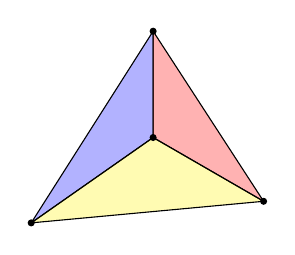
\begin{tikzpicture}
      \def\ds{3}
      \def\pa{(0: 0)}
      \def\pb{(90: \ds)}
      \def\pc{(215: 1.4*\ds)}
      \def\pd{(-30: 1.2*\ds)}

      \def\bcr{3}
      \def\scr{0.55*\bcr}
      \def\sca{34}
      \def\mcr{0.7*\bcr}
      \def\mca{142}
      \def\pr{0.1}

      % Triangles
      \draw[fill=blue,fill opacity=0.3] \pa -- \pb -- \pc -- cycle;
      \draw[fill=red,fill opacity=0.3] \pa -- \pb -- \pd -- cycle;
      \draw[fill=yellow,fill opacity=0.3] \pa -- \pd -- \pc -- cycle;

      % Points
      \fill \pa circle (\pr);
      \fill \pb circle (\pr);
      \fill \pc circle (\pr);
      \fill \pd circle (\pr);
    \end{tikzpicture}
  \end{center}

  It is not possible to make more than $3$ triangles with $4$ points.

  What is the maximum number of non-overlapping triangles that can be made by arranging $290$ points on a plane and drawing non-intersecting lines between them?
}

\def\advent@xxiv@ix{
  Put the digits $1$ to $9$ (using each digit exactly once) in the boxes so that the sums are correct.
  The sums should be read left to right and top to bottom ignoring the usual order of operations.
  For example, $4 + 3 \times 2$ is $14$, not $10$.
  Today's number is the product of the numbers in the red boxes.

  \grid@advent@xxiv@ix{}{}{}{}{}{}{}{}{}
}

\def\advent@xxiv@x{
  A number is a palindrome if it's the same when its digits are written in reverse order.

  What is the sum of all the numbers between $10$ and $100$ that are palindromes?
}

\def\advent@xxiv@xi{
  There are $6$ sets of integers between $1$ and $5$ (inclusive) that contain an odd number of numbers whose median value is $3$:

  \begin{itemize}
    \item $\braces{3}$
    \item $\braces{1,3,4}$
    \item $\braces{2,3,4}$
    \item $\braces{1,3,5}$
    \item $\braces{2,3,5}$
    \item $\braces{1,2,3,4,5}$
  \end{itemize}

  How many sets of integers between $1$ and $11$ (inclusive) are there that contain an odd number of numbers whose median value is $5$?
}

\def\advent@xxiv@xii{
  Holly picks a three-digit number.
  She then makes a two-digit number by removing one of the digits.
  The sum of her two numbers is $309$.
  What was Holly's original three-digit number?
}

\def\advent@xxiv@xiii{
  Today's number is given in this crossnumber.
  No number in the completed grid starts with $0$.

  \begin{multicols}{2}
    \crossnumstd{}{}{}{}{}{}{}{}{}

    \vfill\null
    \columnbreak

    \begin{center}
      \textbf{Across}

      \begin{tabular}{clc}
        \textbf{1} & Today's number.  & (\textbf{3}) \\
        \textbf{4} & Two times 5A.    & (\textbf{3}) \\
        \textbf{5} & A multiple of 1. & (\textbf{3})
      \end{tabular}

      \textbf{Down}

      \begin{tabular}{clc}
        \textbf{1} & Sum of digits is 15. & (\textbf{3}) \\
        \textbf{2} & Sum of digits is 19. & (\textbf{3}) \\
        \textbf{3} & Three times 5A.      & (\textbf{3})
      \end{tabular}
    \end{center}
  \end{multicols}
}

\def\advent@xxiv@xiv{
  $15^3$ is $3375$.
  The last $3$ digits of $15^3$ are $375$.

  What are the last $3$ digits of $15^{1234567890}$?
}

\def\advent@xxiv@xv{
  The number $2268$ is equal to the product of a square number (whose last digit is not $0$) and the same square number with its digits reversed: $36 \times 63$.

  What is the smallest three-digit number that is equal to the product of a square number (whose last digit is not $0$) and the same square number with its digits reversed?
}

\def\advent@xxiv@xvi{
  Put the digits $1$ to $9$ (using each digit exactly once) in the boxes so that the sums are correct.
  The sums should be read left to right and top to bottom ignoring the usual order of operations.
  For example, $4 + 3 \times 2$ is $14$, not $10$.
  Today's number is the product of the numbers in the red boxes.

  \grid@advent@xxiv@xvi{}{}{}{}{}{}{}{}{}
}

\def\advent@xxiv@xvii{
  The number $40$ has $8$ factors: $1$, $2$, $4$, $5$, $8$, $10$, $20$, and $40$.

  How many factors does the number $2^{26} \times 5 \times 7^5 \times 11^2$ have?
}

\def\advent@xxiv@xviii{
  TODO
}

\def\card@xxiv@i{
  What is the largest number you can make by using the digits $1$ to $4$ to make two $2$-digit numbers, then mutiplying the two numbers together?
}

\def\card@xxiv@ii{
  What is the largest number you can make by using the digits $0$ to $9$ to make a $2$-digit number and an $8$-digit number, then mutiplying the two numbers together?
}

\def\card@xxiv@iii{
  The expansion of $(2x+3)^2$ is $4x^2 + 12x + 9$.
  The sum of the coefficients of $4x^2 + 12x + 9$ is $25$.
  What is the sum of the coefficients of the expansion of $(30x + 5)^2$?
}

\def\card@xxiv@iv{
  What is the sum of the coefficients of the expansion of $(2x+1)^{11}$?
}

\def\card@xxiv@v{
  What is the geometric mean of all the factors of $41306329$?
}

\def\card@xxiv@vi{
  What is the largest number for which the geometric mean of all its factors is $92$?
}

\def\card@xxiv@vii{
  What is the sum of all the factors of $7^4$?
}

\def\card@xxiv@viii{
  How many numbers between $1$ and $28988500000$ have an odd number of factors?
}

\def\card@xxiv@ix{
  Eve found the total of the $365$ consecutive integers starting at $500$ and the total of the next $365$ consecutive integers, then subtracted the smaller total from the larger total.
  What was her result?
}

\def\card@xxiv@x{
  Eve found the total of the $n$ consecutive integers starting at a number and the total of the next $n$ consecutive integers, then subtracted the smaller total from the larger total.
  Her result was $22344529$.
  What is the largest possible value of $n$ that she could have used?
}

\input{boxes}

\begin{document}

\title{MS Scroggs Advent Calendar 2021 Answers}
\author{Dan Whitman}
\date{}

\maketitle

Answers: \href{https://www.mscroggs.co.uk/puzzles/advent2021}{https://www.mscroggs.co.uk/puzzles/advent2021}

\aproblem{1}{484}{\advent@xxi@i}{
  We have an unknown, three-digit number $x$ with $n$ factors $f_i$ for $1 \leq i \leq n$.
  From the given geometric mean, we have that
  \gath{
    \prod_{i=1}^n f_i = 22^n = 2^n 11^n \,, \label{eqn:01:prod}
  }
  where we note that $2 \cdot 11$ is the prime factorization of $22$.
  It follows that the factors $f_i$ and, as a result, $x$ itself can only have prime factors of $2$ and $11$.
  Therefore
  \gath{
    x = 2^m 11^k
  }
  for some positive integers $m$ and $k$.
  Moreover, there are
  \gath{
    n = (m+1)(k+1)
  }
  factors of $x$, which we can index as $f_{ij} = 2^i 11^j$ for $(i,j) \in I_m \times I_k$, where $I_n = \braces{0, 1, \ldots, n}$.
  The product of these factors is then
  \ali{
    \prod_{(i,j) \in I_m \times I_k} f_{ij} &= \prod_{i=0}^m \parens{\prod_{j=0}^k f_{ij}} = \prod_{i=0}^m \parens{\prod_{j=0}^k 2^i 11^j} = 2^{\sum_{i=0}^m \sum_{j=0}^k i} 11^{\sum_{i=0}^m \sum_{j=0}^k j} = 2^\frac{m(m+1)(k+1)}{2} 11^\frac{k(k+1)(m+1)}{2} \non
    &= 2^n 11^n
  }
  from \eqref{eqn:01:prod}.
  It follows from this that
  \gath{
    n = \frac{m(m+1)(k+1)}{2} = \frac{k(k+1)(m+1)}{2} \label{eqn:01:km} \\
    m = k \,.
  }
  So it seems that $x = 2^m 11^m$ and hence the number of factors becomes
  \gath{
    n = (m+1)^2 \,. \label{eqn:01:nm}
  }
  Combining \eqref{eqn:01:km} and \eqref{eqn:01:nm} gives
  \gath{
    n = (m+1)^2 = \frac{m(m+1)(k+1)}{2} = \frac{m(m+1)^2}{2} \non
    1 = \frac{m}{2} \non
    m = 2 \,.
  }
  Therefore $x = 2^m 11^m = 2^2 11^2 = 4 \cdot 121 = 484$.
  This result was verified with Python.
}

\aproblem{2}{144}{\advent@xxi@ii}{
For a general number $x$ with a prime factorization
\gath{
x = \prod_{i=1}^m p_i^{e_i}
}
into $m$ distinct primes, the number of factors of $x$ is
\gath{
  N(x) = \prod_{i=1}^m (e_i + 1) \,,
}
which includes counting $1$ and $x$ itself.
Note that, whenever $m > 1$, this must be a composite number.
However, we are told that $7n$ has $37$ factors, and $37$ is prime.
Hence it has to be that $7n$ has only a single prime factor.
Moreover, since clearly $7$ is a prime factor of $7n$, it must be that it is the only prime factor so that in fact $n = 7^{35}$ so that $N(7n) = N(7^{36}) = 36 + 1 = 37$.
Hence we have that we have the prime factorization
\gath{
  8n = 8 \cdot 7^{35} = 2^3 7^{35}
}
and thus
\gath{
  N(8n) = (3+1)(35+1) = 4 \cdot 36 = 144 \,,
}
which must be our answer.
}

\aproblem{3}{192}{
  \advent@xxi@iii
}{
  In the following let $d$ denote a digit from $1$ to $9$.
  We enumerate classes of numbers from $1$ to $1000$ that have zeros and count the zeros that appear in each class:
  \begin{center}
    \begin{tabular}{c|c}
      Class  & Total Zeros      \\
      \hline
      $d0$   & $9$              \\
      $d00$  & $9\cdot 2 = 18$  \\
      $dd0$  & $9 \cdot 9 = 81$ \\
      $d0d$  & $9 \cdot 9 = 81$ \\
      $1000$ & $3$
    \end{tabular}
  \end{center}
  Note that no zeros appear in any single digit numbers since we start at $1$ and not $0$.
  Therefore we would count a total of $9 + 18 + 81 + 81 + 3 = 192$ zeros.
  This result was verified with a brute force Python program.
}

\aproblem{4}{160}{\advent@xxi@iv}{
  \boxans{\gridsol@advent@xxi@iv}
}

\aproblem{5}{240}{\advent@xxi@v}{
  Suppose that a general isosceles triangle has two sides of length $a$ and a third side (the base) of length $b$, with a height of $h$.
  The perimeter is of course
  \gath{
    p = 2a + b
  }
  so that
  \gath{
    a = \frac{p - b}{2} \,. \label{eqn:05:a}
  }
  Also, clearly the lengths are related as right triangles by
  \gath{
    \parens{\frac{b}{2}}^2 + h^2 = a^2
  }
  so that, substituting \eqref{eqn:05:a},
  \gath{
    h = \sqrt{a^2 - \frac{b^2}{4}} = \sqrt{\parens{\frac{p - b}{2}}^2 - \frac{b^2}{4}} = \frac{1}{2} \sqrt{p(p - 2b)} \,.
  }
  The area of the triangle as a function of the base is then
  \gath{
    A(b) = \frac{bh}{2} = \frac{b \sqrt{p(p - 2b)}}{4} \,.
  }
  Now, clearly this is defined only when the term under the radical is non-negative, that is
  \gath{
    p(p - 2b) \geq 0 \non
    p - 2b \geq 0 \non
    b \leq \frac{p}{2} \,,
  }
  noting that of course $p > 0$.
  Since $A(0) = A(p/2) = 0$ is an invalid area, the only isosceles triangles that exist with perimeter $p$ are when $0 < b < p/2$.
  Below is a plot of $A(b)$ for this range of $b$ for $p = 50$ as given:

  \begin{center}
    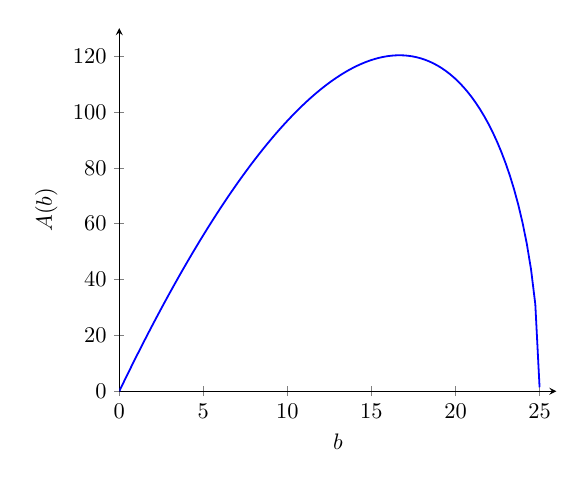
\begin{tikzpicture}[scale=1.8]
      \begin{axis}[
          axis lines=left,
          xmin=0, xmax=26,
          ymin=0, ymax=130,
          xlabel=\(b\),
          ylabel=\(A(b)\),
          samples=100,
        ]
        \addplot[
          blue,
          thick,
          domain=0:25,
        ]
        {x*sqrt(50*(50 - 2*x))/4};
      \end{axis}
    \end{tikzpicture}
  \end{center}

  Clearly there is a maximum here, which can be found as follows:
  \gath{
    \deriv{A}{b} = \deriv{}{b} \frac{b \sqrt{p(p - 2b)}}{4} = \frac{\sqrt{p(p - 2b)}}{4} - \frac{b(-2p)}{8\sqrt{p(p - 2b)}} = \frac{p(p - 3b)}{4 \sqrt{p(p - 2b)}} = 0 \non
    p - 3b = 0 \non
    b = \frac{p}{3} \,.
  }
  The maximum area is then
  \gath{
    A(p/3) = \frac{\frac{p}{3} \sqrt{p(p - 2\frac{p}{3})}}{4} = \frac{p^2}{12 \sqrt{3}} \approx 120.28
  }
  for $p = 50$.
  Thus, for each area where $0 < A < 120.28$, there are two isosceles triangles (one where $0 < b < p/3$ and another where $p/3 < b < p/2$) with that area.
  Clearly there are $120$ integer areas in this range so that there are $2 \cdot 120 = 240$ triangles with integer areas.
}

\aproblem{6}{607}{\advent@xxi@vi}{
  Let $x$ be today's number.
  Then, from what is given, we clearly have a system of modulo equations:
  \ali{
    12345 &\equiv 205 \pmod{x} \\
    6789 &\equiv 112 \pmod{x} \,.
  }
  However, since the unknown is the modulo value, the Chinese Remainder Theorem cannot be used, so we take a more direct approach.
  From the above, we clearly have
  \gath{
    nx + 205 = 12345 \\
    mx + 112 = 6789
  }
  for some positive integers $n$ and $m$.
  Therefore
  \gath{
    (nx + 205) - (mx + 112) = 12345 - 6789 = 5556 \non
    x(n - m) = 5463 \,.
  }
  So $x$ is a factor of $5463$.
  This has factors of $\braces{1, 3, 9, 607, 1821, 5463}$.
  Fortunately for us, only one of these is three digits, which must be our answer!
  The original congruence equations for $x = 607$ were verified with Python.
}

\aproblem{7}{240}{\advent@xxi@vii}{
  First, set the origin of a coordinate system to the center of the decagon.
  Then there are two points at the bottom at $y = -b_2$, two at $y = -b_1$, the middle two at $y = 0$, two at $y = b_1$, and the top two at $y = b_2$, where $0 < b_1 < b_2$.
  Consider first the following triangle, which is one of the ten congruent segments of the decagon:
  \begin{center}
    \begin{tikzpicture}
      \def\dr{2}
      \decagon{0}{0}{\dr}{0}{0}
    \end{tikzpicture}
  \end{center}
  The area of the decagon is clearly ten times the area of this triangle, that is
  \gath{
    A_d = 10 \frac{1}{2} s b_2 = 5 s b_2 \,,
  }
  where we have let $s$ be the length of the sides.
  Thus, clearly
  \gath{
    s = \frac{A_d}{5 b_2} \,. \label{eqn:07:s}
  }
  Now, if we number the decagons with the different triangles in the original question from $1$ to $8$ from left to right and top to bottom, then, by symmetry, clearly the area of  $1$ is the same as that of triangle $8$.
  Similarly, the area of triangle $2$ is the same as the area of triangle $7$, and so on and so forth.
  These areas are then reasoned to be
  \ali{
    A_{1,8} &= \frac{1}{2}s(-b1 - (-b_2)) = \frac{1}{2}s(b_2 - b_1) \\
    A_{2,7} &= \frac{1}{2}s(0 - (-b_2)) = \frac{1}{2} s b_2 \\
    A_{3,6} &= \frac{1}{2}s(b_1 - (-b_2)) = \frac{1}{2} s (b_1 + b_2) \\
    A_{4,5} &= \frac{1}{2}s(b_2 - (-b_2)) = s b_2 \,.
  }
  Therefore the total area of all of the triangles is
  \ali{
    A &= 2A_{1,8} + 2A_{2,7} + 2A_{3,6} + 2A_{4,5} \non
    &= s(b_2 - b_1) + s b_2 + s (b_1 + b_2) + 2 s b_2 \non
    &= s b_2 - s b_1 + s b_2 + s b_1 + s b_2 + 2s b_2 \non
    &= 5 s b_2 = 5 b_2 \frac{A_d}{5 b_2} \non
    &= A_d \,,
  }
  where we have substituted in \eqref{eqn:07:s}.
  Hence evidently this area is simply the area of the decagon!
}

\aproblem{8}{418}{\advent@xxi@viii}{
  The prime factorization of 836 is
  \gath{
    836 = 2^2 \cdot 11 \cdot 19 \,,
  }
  that is we have the four prime factors $2$, $2$, $11$, and $19$.
  We must choose two of these to multiply together to reduce these to our three factors.
  There are only four ways to do this, which are shown below with their respective sums:
  \ali{
    2 + 2 + 11 \cdot 19 &= 213 \\
    2 \cdot 2 + 11 + 19 &= 34 \\
    2 + 2 \cdot 11 + 19 &= 43 \\
    2 + 11 + 2 \cdot 19 &= 51 \,.
  }
  Clearly the last of these are the factors we seek, so that our answer is $2 \cdot 19 \cdot 11 = 418$.
}

\aproblem{9}{102}{\advent@xxi@ix}{
  First, if $a \geq 0$ and $n \geq 1$ are integers, then the sum of the $n$ consecutive integers starting at $a$ is
  \ali{
    \sum_{k=a}^{a+n-1} k &= \sum_{k=1}^{a+n-1} k - \sum_{k=1}^{a-1} k = \frac{(a+n-1)(a+n)}{2} - \frac{(a-1)a}{2} \non
    &= \frac{1}{2}\parens{a^2 + an + an + n^2 - a - n - a^2 + a} \non
    &= \frac{1}{2}\parens{n^2 + 2an - n} \non
    &= \frac{1}{2}n\parens{n + 2a - 1} \,.
  }
  Now, in our case the sum of such consecutive numbers is $844$, the prime factorization of which is
  \gath{
    844 = 2^2 \cdot 211 \,.
  }
  Thus, for unknown positive integers $a$ and $n$, we have that the consecutive sum is
  \gath{
    \sum_{k=a}^{a+n-1} k = \frac{1}{2}n\parens{n + 2a - 1} = 844 = 2^2 \cdot 211 \non
    n(n + 2a - 1) = 2^3 \cdot 211 \,.
  }
  Now, clearly $n + 2a - 1 > n$ since $a > 0$, from which it follows that the $211$ must be contained in the $n + 2a - 1$ factor since otherwise we would have $n \geq 211$ and $n + 2a - 1 \leq 2^3 = 8$, since that is the remaining factor, and thus $n \geq 211 > 8 \geq n + 2a - 1$.
  Moreover, letting $b = 2^3 \cdot 211$, we have that
  \gath{
    n(n + 2a - 1) = b \non
    2a = \frac{b}{n} - n + 1 \,.
  }
  Since the left side of this is even, the right must be as well.
  Since $n$ cannot contain the $211$, it must be that $n = 2^k$ for some $1 \leq k \leq 3$, noting that we are told that she writes more than one number so that $n > 1$ and hence $k \geq 1$.
  Thus $n$ is even so that $-n + 1$ is odd so that, for the right side to be even, it must be that $b/n$ must be odd.
  Since $b = 2^3 \cdot 211$, this will only be the case if $n= 2^3 = 8$, and hence
  \gath{
    a = \frac{1}{2}\parens{\frac{b}{n} - n + 1} = 102 \,,
  }
  which is our answer.
  Indeed we find that we have the sum of the $n = 8$ integers $102 + 103 + 104 + 105 + 106 + 107 + 108 + 109 = 844$ as required.
}

\aproblem{10}{654}{\advent@xxi@x}{
  \boxans{\gridsol@advent@xxi@x}
}

\aproblem{11}{696}{\advent@xxi@xi}{
  If we number the rows starting at $1$ at the top (for the row containing only $1$) going down, then clearly the number of elements in the $n$th row is $N(n) = 2n - 1$.
  Let $a_n$ be the \emph{first} number in the $n$th row.
  It is then reasoned that $a_1 = 1$ along with the recursive relationship
  \gath{
    a_n = a_{n-1} + N(n-1) = a_{n-1} + 2(n-1) - 1 = a_{n-1} + 2n - 3 \label{eqn:11:rec}
  }
  defines the sequence $\angles{a_n}$.
  Moreover, it was reasoned that a closed form for $a_n$ is
  \gath{
    a_n = n(n - 2) + 2 \,, \label{eqn:11:an}
  }
  which is easily proven.
  First, clearly $a_1 = 1(1-2) + 2 = -1 + 2 = 1$ as required.
  If we assume that \eqref{eqn:11:an} is true for $n$, then, by the recursion relation \eqref{eqn:11:rec}, we have
  \ali{
    a_{n+1} &= a_n + 2(n+1) - 3 = \squares{n(n - 2) + 2} + 2n + 2 - 3 = n^2 - 2n + 2n + 1 \non
    &= n^2 + 1 = n^2 - 1 + 2 = (n+1)(n-1) + 2 \non
    &=(n+1)(\squares{n+1} - 2) + 2 \,,
  }
  which shows the result by induction.
  It is also reasoned that, for a number $a$ in the $n$th row, the number directly above it is $a - 2(n-1)$, except the first and last numbers, which have nothing above them.
  Now, using \eqref{eqn:11:an}, we have that $a_{28} = 730$ whereas $a_{29} = 785$, which means that $a = 750$ is somewhere in the middle of the $28$th row, i.e. $n = 28$.
  Thus our answer is
  \gath{
    a - 2(n-1) = 750 - 2(28 - 1) =  696 \,.
  }
}

\aproblem{12}{120}{\advent@xxi@xii}{
  The Dec~9 problem from the 2015 advent calendar was the same problem except that the grid there was a larger $5 \times 7$ instead of our $3 \times 7$ grid.
  Again let $N(h, w)$ denote the number of routes from the lower left corner of a $h \times w$ (height by width) grid to the upper right corner.
  Using the same method as before, and using the partial results of that derivation, we have that
  \gath{
    N(3, w) = \sum_{a=0}^w \sum_{b=0}^a \sum_{c=0}^b 1 = \frac{1}{6} \squares{w^3 + 6w^2 + 11w + 6}
  }
  for a $3 \times w$ grid.
  Hence our answer is $N(3, 7) = 120$.
  This was also verified using the same Python code that implements the recursive solution.
}

\aproblem{13}{904}{\advent@xxi@xiii}{
First, suppose that we have two line segments of length $a$ and $b$ that intersect at their endpoints, meeting at an angle $\phi$.
Set the origin to the intersection point with the positive $x$-axis aligning to the segment of length $a$.
Then the endpoints of each line segment are clearly
\ali{
  p_a &= (a, 0) &
  p_b &= (b \cos{\phi}, b \sin{\phi})
}
Thus the distance between these endpoints is
\ali{
\abs{p_b - p_a} &= \abs{(b \cos{\phi} - a, b \sin{\phi} - 0)} = \sqrt{(b \cos{\phi} - a)^2 - (b \sin{\phi})^2} \non
&= \sqrt{b^2 \cos^2{\phi} - 2 a b \cos{\phi} + a^2 + b^2 \sin^2{\phi}} \non
&= \sqrt{b^2 - 2 a b \cos{\phi} + a^2}
}
Now, if we scale both of these line segments by a factor $\a > 0$, then this distance scales by the same amount:
\ali{
\abs{\a p_b - \a p_a} &= \abs{(\a b \cos{\phi} - \a a, \a b \sin{\phi} - \a \cdot 0)} = \sqrt{(\a b \cos{\phi} - \a a)^2 - (\a b \sin{\phi})^2} \non
&= \sqrt{\a^2 (b^2 \cos^2{\phi} - 2 a b \cos{\phi} + a^2) + \a^2 b^2 \sin^2{\phi}} \non
&= \a \sqrt{b^2 - 2 a b \cos{\phi} + a^2} \non
&= \a \abs{p_b - p_a} \,.
}
To digress momentarily, if we have a triangle with base $b$ and height $h$, clearly its area is $A_1 = bh/2$.
If the sides of the triangle all scale by $\a > 0$ then of course the base becomes $\a b$ and the height $\a h$ so that the area becomes
\gath{
  A = \frac{1}{2}(\a b)(\a h) = \a^2 \frac{1}{2} b h = \a^2 A_1 \,,
}
that is the area scales by $\a^2$.
Now, for our problem, the center and diameter points of each circle both lie on the same line, and the three lines intersect at a common point.
Each side of the red triangle is the pairwise distance between the center points.
Each side of the blue triangle, on the other hand, is the pairwise distance between the diameter points.
Therefore, by what was shown above, since the diameter points are twice as far from the intersection point as the center points, the blue triangle is similar to the red triangle where the sides scale by a factor of two.
Thus the area scales by a factor of $2^2 = 4$ so that our answer is
\gath{
  A_\mathrm{blue} = 4 A_\mathrm{red} = 4 \cdot 226 = 904 \,.
}
}

\aproblem{14}{512}{\advent@xxi@xiv}{
  Adapting the analytical approach of the Dec~12 problem to this additional freedom results in a simpler solution.
  Again consider the number of spaces to the right of the path in each row.
  Since we can move to the left, now instead of the possible number of spaces right of the path in a row depending on the number of spaces to the right in the row below, they are now independent.
  In each row then the number of spaces to the right of the path can be any number from $0$ to $w$ for a $h \times w$ grid regardless of the rows below, i.e. there are $w+1$ possibilities.
  Hence the total number of paths simply becomes
  \gath{
    N(h, w) = (w + 1)^h \,.
  }
  Previously, without being able to move left, there was the symmetry in that $N(h, w) = N(w, h)$, but now that is not the case since we can move in two directions horizontally but only in one vertically.
  Hence in our problem we have
  \gath{
    N(3, 7) = (7 + 1)^3 = 8^3 = 512 \,.
  }
  However, the recursive approach derived in the Dec~12 problem can no longer be described in terms of a simple recursive function.
  Rather, an algorithm is needed in which we keep a set of visited nodes $V$.
  We again use the convention that the lower left corner is node $(h, w)$ and the upper right corner is node $(0, 0)$.
  As our kind of base case, we say that $N(y, x) = 0$ if either $(y, x) \in V$, since these are nodes where we have already been, or if $(y, x)$ is out of bounds of the grid, i.e. if $x < 0$, $x > w$, $y < 0$, or $y > h$.
  At our destination, we also have $N(0, 0) = 1$.
  At the current node $(y, x)$, we add $(y, x)$ to $V$ and then recurse with
  \gath{
    N(y, x) = N(y-1, x) + N(y, x+1) + N(y, x-1)
  }
  since we can move up, left, or right.
  We of course then evaluate $N(h, w)$ recursively.
  Implementing and running this algorithm in Python gives the same answer as above for $N(3, 7)$.
}

\aproblem{15}{361}{\advent@xxi@xv}{
  First, clearly each of the numbers in the pyramid is $2k+1$ where the corresponding values of $k$ form the following pyramid:

  \pyramid@advent@xxi@xv{0}{1}{2}{3}{4}{5}

  In \emph{this} pyramid, the first number $a_n$ in row $n$ satisfies $a_1 = 0$ along with the the recursive relationship
  \gath{
    a_n = a_{n-1} + n - 1 \,.
  }
  It was reasoned then that, in closed form,
  \gath{
    a_n = \frac{n(n-1)}{2} \,. \label{eqn:15:an}
  }
  This is trivial to prove by induction since $a_1 = (1 \cdot 0) /2 = 0$ and, if we assume \eqref{eqn:15:an} for $n$, we have
  \gath{
    a_{n+1} = a_n + (n+1) - 1 = \frac{n(n-1)}{2} + n = \frac{n^2 - n + 2n}{2} = \frac{n^2 + n}{2} = \frac{n(n+1)}{2} = \frac{(n+1)\squares{(n+1) - 1}}{2} \,.
  }
  Clearly the $n$th row of both pyramids has $n$ elements, with the difference between each element in the \emph{original} pyramid being $2$.
  It then follows that the mean of the $n$th row of the original pyramid is simply
  \ali{
    \mu_n &= \frac{1}{n} \sum_{k=0}^{n-1} (2a_n + 1 + 2k) = \frac{1}{n}\squares{\sum_{k=0}^{n-1} (2a_n + 1) + 2 \sum_{k=0}^{n-1} k} \non
    &= \frac{1}{n} \squares{n(2a_n + 1) + 2\frac{n(n-1)}{2}} = 2a_n + 1 (n - 1) \non
    &= 2a_n + n = 2 \frac{n(n-1)}{2} + n = n^2 - n + n \non
    &= n^2 \,,
  }
  where we have of course substituted in \eqref{eqn:15:an} along the way.
  Therefore our answer is $\mu_{19} = 19^2 = 361$.
  This was also verified with Python using brute force.
}

\aproblem{16}{222}{\advent@xxi@xvi}{
  Logic was used to deduce the solution:

  \crossnumstd{2}{5}{2}{2}{1}{6}{2}{2}{1}

  Python was used to verify this solution.
}

\aproblem{17}{479}{\advent@xxi@xvii}{
  The prime factorization of $252$ is
  \gath{
    252 = 2^2 3^2 7
  }
  so that all these factors must be present in any number whose digital product is $252$.
  To find the smallest such number, we clearly want to use a few digits as possible.
  The $7$ cannot be used to make any other digits, so the answer must contain a $7$.
  However, the digit $4$ can be used to cover the $2^2$ instead of two \mn{2}, and a $9$ can be used to cover the $3^2$ rather than two \mn{3}.
  We could alternatively cover $2^2 3^2$ using two \mn{6}, but this would result in a larger number than using the $4$ and $9$.
  Hence our answer is $479$, which was verified with Python using brute force.
}

\aproblem{18}{432}{\advent@xxi@xviii}{
  \boxans{\gridsol@advent@xxi@xviii}
}

\aproblem{19}{175}{\advent@xxi@xix}{
  For a general cubic equation
  \gath{
    \a x^3 + \b x^2 + \g x + \d = 0 \,,
  }
  its discriminant is
  \gath{
    \D = 18 \a \b \g \d - 4 \b^3 \d + \b^2 \g^2 - 4 \a \g^3 - 27 \a^2 \d^2 \,. \label{eqn:19:Do}
  }
  In our case we clearly have
  \ali{
    \a &= 352 & \g &= 0 \\
    \b &= -528 & \d &= a
  }
  so that \eqref{eqn:19:Do} becomes
  \gath{
    \D = -4 \b^3 a - 27 \a^2 a^2
  }
  Now, there are three \emph{distinct} real solutions when and only when $\D > 0$ so that we have
  \gath{
    \D = -4 \b^3 a - 27 \a^2 a^2 > 0 \non
    - 27 \a^2 a^2 > 4 \b^3 a \non
    a^2 < \frac{-4 \b^3}{27 \a^2}a = 176a \label{eqn:19:ineq}
  }
  since of course $\a^2 > 0$ so that $-27 \a^2 < 0$.
  We are told that $a$ can be \emph{any} integer (i.e. not necessarily positive), so we must treat three separate cases.
  First, if $a = 0$, then \eqref{eqn:19:ineq} becomes $0 > 0$ and so is not satisfied.
  Hence $a = 0$ does not does not result in three distinct roots.
  If $a > 0$ then we can divide both sides of \eqref{eqn:19:ineq} by $a$ to get
  \gath{
    0 < a < 176 \,.
  }
  Clearly there are exactly $175$ integers that satisfy this condition.
  Lastly, if $a < 0$ then we can still divide both sides of \eqref{eqn:19:ineq} by $a$, but we need to the inequality to get
  \gath{
    a > 176 \,.
  }
  As there are no integers for which both $a < 0$ and $a > 176$, this case contributes no solutions of interest.
  Therefore our final answer is simply $175$.
}

\aproblem{20}{304}{\advent@xxi@xx}{
  First, a triangle is valid only when the pairwise sum of any two sides is greater than the third side.
  Suppose that $a$ is an unknown side of interest, and $b = 19$ and $c = 32$ per what was given.
  So it must be that
  \gath{
    a + b > c \non
    a > c - b = 13 \,.
  }
  as well as
  \gath{
    a + c > b \non
    a > b - c = -13 \label{eqn:20:always}
  }
  and
  \gath{
    51 = b + c > a \,.
  }
  Since \eqref{eqn:20:always} is always satisfied, we only have valid triangles for $13 < a < 51$.
  We note that, in the cases where $a = 13$ or $a = 51$, the triangle collapses down into a line with effectively zero area.
  Now, if $a$, $b$, and $c$ are the sides of a general triangle, then Heron's formula gives its area strictly in terms of these sides.
  One of the forms of this is that the area is
  \gath{
    A = \frac{1}{4}\sqrt{(a + b + c)(-a + b + c)(a - b + c)(a + b - c)} \,. \label{eqn:20:heron}
  }
  If we let $\a = b + c$ and $\b = c - b$ then then \eqref{eqn:20:heron} as a function of $a$ becomes
  \ali{
    A(a) &= \frac{1}{4}\sqrt{(a + \a)(-a + \a)(a + \b)(a - \b)} \non
    &= \frac{1}{4}\sqrt{(\a^2 - a^2)(a^2 - \b^2)} \label{eqn:20:Aa}
  }
  A plot of this function is shown below for our $\a = b + c = 51$ and $\b = c - b = 13$:
  \begin{center}
    \begin{tikzpicture}[scale=1.8]
      \begin{axis}[
          axis lines=left,
          xmin=10, xmax=55,
          ymin=0, ymax=350,
          xlabel=\(a\),
          ylabel=\(A(a)\),
          samples=100,
        ]
        \addplot[
          blue,
          thick,
          domain=13:51,
        ]
        {1/4*sqrt((51^2 - x^2)*(x^2 - 13^2))};
      \end{axis}
    \end{tikzpicture}
  \end{center}
  Note that, as expected, the area goes to zero at $a = 13$ and $a = 51$.
  Also note that the area has a maximum value, which is the answer we seek.
  To find this, we of course set
  \gath{
    \deriv{A}{a} = \frac{-2a(a^2 - \b^2) + 2a(\a^2 - a^2)}{8\sqrt{(\a^2 - a^2)(a^2 - \b^2)}} = \frac{a(\a^2 + \b^2 - 2a^2)}{8\sqrt{(\a^2 - a^2)(a^2 - \b^2)}} = 0 \non
    a(\a^2 + \b^2 - 2a^2) = 0
  }
  Since $a = 0$ is outside of our valid region, the maximum must occur at
  \gath{
    \a^2 + \b^2 - 2a^2 = 0 \non
    2a^2 = \a^2 + \b^2 \non
    a^2 = \frac{\a^2 + \b^2}{2} = \frac{(b + c)^2 + (c - b)^2}{2} = \frac{b^2 + 2bc + c^2 + c^2 - 2bc + b^2}{2} = \frac{2b^2 + 2c^2}{2} = b^2 + c^2 \,.
  }
  Note that this resembles the Pythagorean Theorem, indicating that the maximum area seems to occur when $a$ is the length such that the triangle is a right triangle with legs $b$ and $c$ and hypotenuse $a$.
  In any case, substituting $a^2 = b^2 + c^2$ back into \eqref{eqn:20:Aa} gives a maximum area of
  \ali{
    A_\mathrm{max} &= \frac{1}{4}\sqrt{(\a^2 - b^2 - c^2)(b^2 + c^2 - \b^2)} = \frac{1}{4}\sqrt{[(b+c)^2 - b^2 - c^2][b^2 + c^2 - (c - b)^2]} \non
    &= \frac{1}{4}\sqrt{(b^2 + 2bc + c^2 - b^2 - c^2)(b^2 + c^2 - c^2 + 2bc - b^2)} \non
    &= \frac{1}{4}\sqrt{(2bc)(2bc)} = \frac{1}{4}\sqrt{(2bc)^2} = \frac{2bc}{4} \non
    &= \frac{bc}{2}
  }
  since $b$ and $c$ are both positive so that $2bc > 0$.
  This is of course the area of a right triangle with legs $b$ and $c$.
  Therefore our answer is $A_\mathrm{max} = bc/2 = (19 \cdot 32) / 2 = 304$.
}

\aproblem{21}{148}{\advent@xxi@xxi}{
  \boxans{\grid@advent@xxi@xxi{1}{4}{8}{2}{9}{3}{5}{7}{6}}
}

\aproblem{22}{760}{\advent@xxi@xxii}{
  A similar problem was the Dec~6 puzzle in the 2020 advent calendar.
  However, in that problem, a special case was treated that our problem does not fit into, so we cannot really utilize those results.
  In our special case we shall only consider two indistinguishable tokens.
  First consider a $1 \times n$ grid and we want to derive the number of ways the two tokens can be placed on this $N_1(n)$ without being adjacent.
  Since they are indistinguishable, we can place the first token and then assume that the second token is always to the \emph{left} of the first.
  Number the spaces from $1$ to $n$ starting on the left.
  Clearly for the second token to be able to be placed at all (to the left of the first), the first must be placed no further to the left than space number $3$.
  If the first token is on space $k$, then there are $k-2$ spaces on which we could place the second token so that it is to the left of but not adjacent to the first, namely spaces $1$ through $k-2$.
  Therefore the total number of configurations is
  \gath{
    N_1(n) = \sum_{k=3}^n (k - 2) = \sum_{k=1}^{n-2} k = \frac{(n-2)(n-1)}{2} \,.
  }
  Now, for a $2 \times n$ grid, the same adjacent spaces are blocked regardless of whether the token is on the bottom or top row.
  So, for each of the possible $N_1(n)$ configurations, there are $4$ configurations on the $2 \times n$ grid corresponding to the combinations of the two tokens being independently on the bottom or top row.
  Thus the number of valid placements on a $2 \times n$ grid is
  \gath{
    N_2(n) = 4 N_1(n) = 4 \frac{(n-2)(n-1)}{2} = 2(n-2)(n-1) \,.
  }
  Indeed, for the $2 \times 4$ grid in the example, we get $N_2(4) = 2 \cdot 2 \cdot 3 = 12$ as expected.
  For the $2 \times 21$ grid, we get our answer $N_2(21) = 2 \cdot 19 \cdot 20 = 760$.
}

\aproblem{23}{102}{\advent@xxi@xxiii}{
  Let $x_1 = -6$ and $x_2 = 17$ with $y_1 = x_1^2$ and $y_2 = x_2^2$.
  The equation of a line passing through these points is then
  \gath{
    y = (x - x_1)\frac{y_2 - y_1}{x_2 - x_1} + y_1 \,. \label{eqn:23:line}
  }
  To find where this intersects the $y$-axis, we of course simply plug $x = 0$ into \eqref{eqn:23:line}:
  \ali{
    y &= (0 - x_1)\frac{y_2 - y_1}{x_2 - x_1} + y_1 = 0 = x_1 \frac{y_1 - y_2}{x_2 - x_1} + y_1 \non
    &= x_1 \frac{x_1^2 - x_2^2}{x_2 - x_1} + x_1^2 = \frac{x_1(x_1^2 - x_2^2) + x_1^2(x_2 - x_1)}{x_2 - x_1} \non
    &= \frac{x_1^3 - x_1 x_2^2 + x_1^2 x_2 - x_1^3}{x_2 - x_1} = \frac{x_1^2 x_2 - x_1 x_2^2}{x_2 - x_1} \non
    &= \frac{x_1 x_2 (x_1 - x_2)}{x_2 - x_1} = -x_1 x_2 \non
    &= -(-6)17 = 6 \cdot 17 = 102 \,,
  }
  which is our answer.
}

\aproblem{24}{792}{\advent@xxi@xxiv}{
  The prime factorization of $20$ is
  \gath{
    20 = 2^2 5 \,.
  }
  Therefore there are only two options to make $20$ with digits: one $4 = 2^2$ and one $5$, or two \mn{2} and one $5$.
  Suppose that we are interested in $n$-digit numbers where $n \geq 3$.
  First considering the one $4$ and one $5$, we can place one, say the $5$, in any of the $n$ digital positions, and then, for each of those, place the $4$ in any of the remaining $n-1$ positions, with the rest of the positions of course being \mn{1}.
  Hence there are
  \gath{
    N_{4,5}(n) = n(n-1)
  }
  of these $n$-digit numbers.
  If we have two \mn{2} and one $5$, we can do the same thing by placing the $5$ and then the two \mn{2}, but the result needs to be halved since the \mn{2} can be interchanged without changing the number, i.e. each number is counted twice without halving.
  Therefore the number of these number is
  \gath{
    N_{2,2,5}(n) = \frac{n(n-1)(n-2)}{2} \,.
  }
  Therefore the total number of $n$-digit numbers whose product is $20$ is
  \ali{
    N(n) &= N_{4,5}(n) + N_{2,2,5}(n) = n(n-1) + \frac{n(n-1)(n-2)}{2} \non
    &= n(n-1)\parens{1 + \frac{n-2}{2}} = n(n-1)\parens{\frac{2 + (n-2)}{2}} \non
    &= \frac{n^2(n-1)}{2} \,. \label{eqn:24:N}
  }
  Our answer is then
  \gath{
    N(12) = \frac{12^2 11}{2} = 792 \,.
  }
  Equation \eqref{eqn:24:N} was validated against a brute force approach in Python for $3 \leq n \leq 7$, but this approach takes too long to compute for $n > 7$.
}

\end{document}
